% Editorial Results entry point: the order follows the scientific questions.
\subsection{Effects of supervision targets and checkpoint selection}
The primary comparison concerns whether the supported-category vote distribution improves selective predictions beyond preserving the dominant target probability. At 80\% coverage, validation-selected Swin-T models trained with Soft have mean complete-vote disagreement of 23.68\%, compared with 24.06\% for Uniform (Table~\ref{tab:primary}). The paired Soft-minus-Uniform difference is -0.38 pp, with a conditional 95\% interval of [-0.64, -0.07]. This is a modest advantage over the matched softening control; each model selects its own accepted images.
\begin{table}[t]
\caption{Selected-checkpoint risk at 80\% coverage (2,620 of 3,275 images). Risk is mean $\pm$ sample SD; components are mean percentage points}\label{tab:primary}
\centering\begin{tabular}{lrrrr}\toprule
Targets & Risk (\%) & Unsupported & Ambiguity & Excess\\\midrule
Hard & $26.30 \pm 1.04$ & 6.65 & 16.14 & 3.51\\
Tie-hard & $25.82 \pm 0.58$ & 6.67 & 16.03 & 3.13\\
Uniform & $24.06 \pm 0.10$ & 6.41 & 15.41 & 2.24\\
Tie-Uniform & $24.27 \pm 0.17$ & 6.47 & 15.46 & 2.35\\
Soft & $23.68 \pm 0.07$ & 6.55 & 15.01 & 2.13\\
\bottomrule\end{tabular}\par
Accepted identities differ; components provide accounting, not causal attribution.
\end{table}


The retained comparisons with hard targets show why the control matters. Soft minus Hard is -2.61 pp (conditional 95\% interval [-2.98, -2.19]), substantially larger than the primary Soft-minus-Uniform contrast. Tie-hard minus Hard is -0.47 pp (interval [-0.80, -0.12]), while Soft minus Tie-hard is -2.14 pp (interval [-2.49, -1.76]). These secondary intervals describe sensitivity to the target construction, rather than additional primary hypothesis tests.

The direction of the primary Swin-T contrast persists when the checkpoint is retained after 12 epochs instead of selected by validation distance. Soft minus Uniform is then -0.32 pp (conditional 95\% interval [-0.63, -0.05]); Soft minus Hard is -1.35 pp (interval [-1.72, -1.05]). Table~\ref{tab:sensitivity} reports the absolute risks at both checkpoint states. This comparison changes checkpoint selection, not the training budget or objective.
\begin{table}[t]
\caption{Selected versus fixed epoch-12 complete-vote risk at 80\% coverage (\%); means across three paired seeds}\label{tab:sensitivity}
\centering\begin{tabular}{lrr}\toprule
Targets & Selected & Epoch 12\\\midrule
Hard & 26.295 & 24.983\\
Tie-hard & 25.824 & 24.576\\
Uniform & 24.062 & 23.949\\
Tie-Uniform & 24.272 & 23.939\\
Soft & 23.684 & 23.632\\
\bottomrule\end{tabular}\par

\end{table}


The tie-preserving control gives the same qualitative result for Swin-T. Soft has lower disagreement than Tie-Uniform at both checkpoint states, with conditional intervals below zero (Table~\ref{tab:backbones}). Unlike Uniform, Tie-Uniform does not favor a single category when the highest vote counts are tied. Both controls nevertheless differ from Soft in entropy and aggregate class proportions, so these comparisons do not isolate the effect of minority-category identity alone. The supplementary learning and selection curves retain all training trajectories; loss magnitudes across different target constructions are not directly comparable measures of fitting quality.

Figure~\ref{fig:difference} places the primary endpoint in the broader coverage range. It is a descriptive comparison using each model's own confidence ranking, not an additional confirmatory test.
\begin{figure}[tp]\centering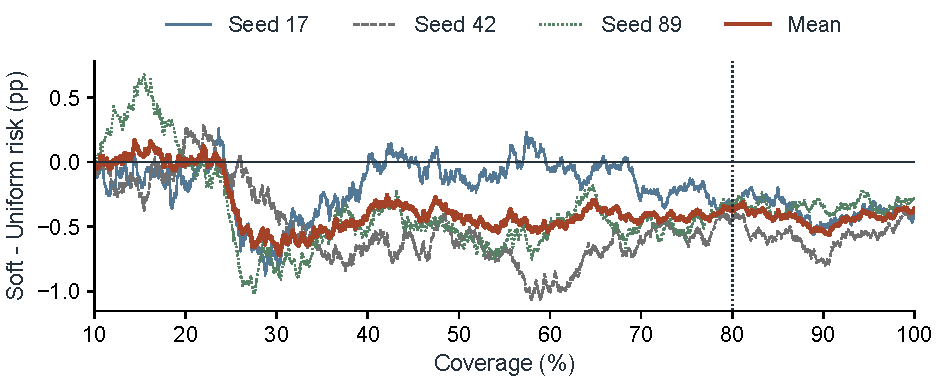
\includegraphics[width=\linewidth]{submission_reader_2026_10_13/source/figures/Fig5.pdf}
\caption{Soft-minus-Uniform complete-vote disagreement versus common coverage. Thin curves show paired seeds; the thick curve shows their mean. Each model uses its own ranking, rather than an identical accepted-image set. The vertical marker identifies the primary 80\% endpoint. No simultaneous uncertainty band is estimated}\label{fig:difference}\end{figure}

\subsection{Distributional agreement and backbone sensitivity}\label{sec:distance}

The secondary distributional endpoint gives a more consistent result than selective category disagreement. Soft has lower squared distance than both controls in every tested seed, backbone and checkpoint state (Table~\ref{tab:distance}). For validation-selected Swin-T, mean distance is 0.09783 for Soft and 0.11571 for Uniform. This endpoint evaluates the complete probability vector on all 3,275 primary-test images, without confidence rejection. Supplementary Sect.~S2 provides the per-seed values for all five Swin-T and three ResNet-18 targets.

\begin{table}[t]\caption{Agreement with the complete crowd-vote distribution. Ten-category squared distances are averaged across three separate seeds on the same 3,275 test images. Lower is better; values are unscaled distance units, not percentages}\label{tab:distance}

\centering\small\begin{tabular}{llrrrrr}\toprule

Backbone & State & Soft & Uniform & Tie-Uniform & $\Delta_U$ & $\Delta_{TU}$\\\midrule

Swin-T & Selected & 0.09783 & 0.11571 & 0.11373 & -0.01787 & -0.01589\\

Swin-T & Epoch 12 & 0.09779 & 0.11699 & 0.11280 & -0.01920 & -0.01501\\

ResNet-18 & Selected & 0.11059 & 0.12303 & 0.11805 & -0.01244 & -0.00746\\

ResNet-18 & Epoch 12 & 0.11089 & 0.12259 & 0.11665 & -0.01170 & -0.00576\\

\bottomrule\end{tabular}\par\smallskip

$\Delta_U$ and $\Delta_{TU}$ are Soft minus Uniform and Soft minus Tie-Uniform. For each image, the score sums ten squared probability differences after adding three zero entries to the seven model outputs. It then averages across images. Vote distributions are not renormalized to the supported categories. Model probabilities are not combined across seeds.\par\end{table}

The adaptive ResNet-18 checks distinguish this distributional advantage from the selective result. For validation-selected ResNet-18, Soft-minus-Uniform disagreement is +0.173 pp, compared with -0.378 pp for Swin-T. All four ResNet-18 conditional intervals cross zero (Table~\ref{tab:backbones}), so these checks do not confirm Swin-T's selective advantage. Supplementary Sect.~S2 reports the per-seed contrasts and accompanying diagnostics. These are architecture-sensitivity checks using the same source images and adaptive study design, not independent-image confirmation.
\begin{table}[t]
\caption{Within-backbone Soft-minus-control disagreement at 80\% coverage (percentage points). Intervals condition on fitted models, three seeds, observed pixels and votes}\label{tab:backbones}
\centering\begin{tabular}{lllrr}\toprule
Backbone & State & Control & Difference & 95\% interval\\\midrule
Swin-T & selected & Uniform & -0.378 & [-0.644, -0.073]\\
Swin-T & selected & Tie-Uniform & -0.588 & [-0.830, -0.281]\\
Swin-T & epoch12 & Uniform & -0.317 & [-0.626, -0.050]\\
Swin-T & epoch12 & Tie-Uniform & -0.307 & [-0.585, -0.024]\\
ResNet-18 & selected & Uniform & +0.173 & [-0.167, +0.455]\\
ResNet-18 & selected & Tie-Uniform & +0.042 & [-0.258, +0.343]\\
ResNet-18 & epoch12 & Uniform & +0.170 & [-0.157, +0.467]\\
ResNet-18 & epoch12 & Tie-Uniform & +0.190 & [-0.126, +0.515]\\
\bottomrule\end{tabular}\par
\smallskip
ResNet comparisons are adaptive secondary robustness checks, not independent-image confirmation or architecture comparisons.\par
\end{table}


Figure~\ref{fig:backbones} brings the two endpoints together. Squared distance measures agreement across the complete annotation distribution, whereas category disagreement depends on the predicted category and, under confidence selection, the accepted-image set. Better distributional agreement can therefore coexist with little or no selective category advantage. The result concerns the tested source-dataset configurations; it does not establish deployment calibration or better external transfer.
\begin{figure}[tp]\centering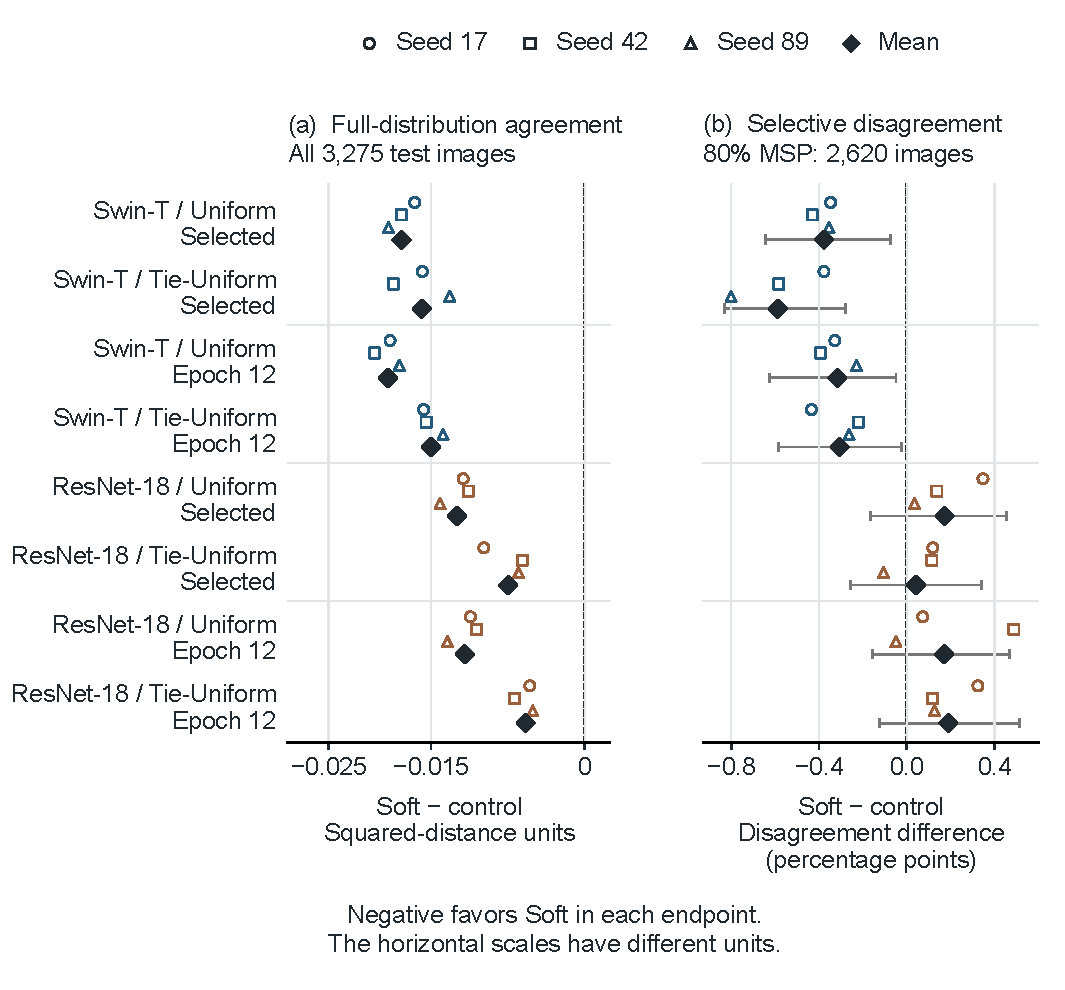
\includegraphics[width=\linewidth]{submission_reader_2026_10_13/source/figures/Fig7.pdf}
\caption{Distributional agreement and selective disagreement for Soft relative to the matched controls. (a) Ten-category squared-distance differences on all 3,275 primary-test images, in unscaled distance units. (b) Complete-vote disagreement differences at 80\% coverage using each model's ranking, in percentage points. Symbols show the three paired-seed contrasts and their mean. Bars in (b) are 95\% pixel-cluster bootstrap intervals conditional on the fitted models and observed votes; no interval is shown in (a). Both backbones and validation-selected and epoch-12 checkpoints are included. Negative values favor Soft. The panels use different units and scales}\label{fig:backbones}\end{figure}


\subsection{Accepted-image sets and annotation references}
For validation-selected Swin-T, the predictor comparison depends on the accepted-image set. Soft-minus-Uniform disagreement is +0.085 pp on images selected by Uniform, but -0.352 pp on images selected by Soft (Fig.~\ref{fig:cross}). Each within-column comparison holds the images and annotation reference fixed, so the difference reflects the predictors' category choices on that set. Lower risk under Soft's own ranking therefore does not establish consistently better category predictions on identical images.
\begin{figure}[tp]\centering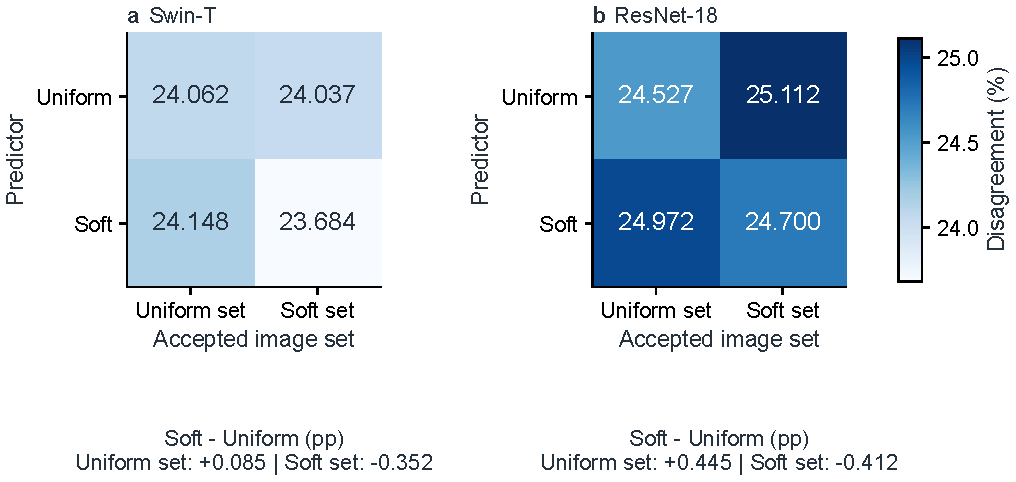
\includegraphics[width=\linewidth]{submission_reader_2026_10_13/source/figures/Fig4.pdf}
\caption{Fixed-image cross-evaluation at 80\% coverage for validation-selected (a) Swin-T and (b) ResNet-18 checkpoints. Cells are complete-vote disagreement percentages averaged across three seeds. Columns fix the selector's 2,620-image set; rows change the predictor. The common color scale shows absolute risk, and signed differences below each panel show within-column Soft-minus-Uniform contrasts. Each model's own-set risk uses a different accepted set}\label{fig:cross}\end{figure}

Changing the accepted set also changes the result for a fixed predictor. Moving from Uniform-selected to Soft-selected images gives a risk change of -0.025 pp for the Uniform predictor and -0.463 pp for the Soft predictor. The mean Jaccard overlap is 0.8408. The ResNet-18 Soft-minus-Uniform comparison likewise changes sign between Uniform-selected (+0.445 pp) and Soft-selected images (-0.412 pp). These patterns show an interaction between prediction and selection rather than a unique causal contribution from either. The supplement retains every seed, both checkpoint states, the complete cross-evaluation matrices and overlap counts.

Changing the annotation reference altered the measured classification performance without changing the predictions. On the same 2,484 supported-majority images, validation-selected Swin-T models trained with Soft had mean weighted F1 of 0.6685 against the original FER2013 labels and 0.9270 against the crowd-majority labels (Table~\ref{tab:samef1}). Image selection also affected the score: under the original FER2013 reference, weighted F1 increased from 0.5722 on all 3,275 primary-test images to 0.6685 on this subset. The first comparison changes the label reference while holding images fixed; the second changes the image population while retaining the original reference. The crowd-majority score therefore describes a different evaluation task from original-label performance on the complete test population, not an improvement in the underlying predictions. The supplementary reference matrix documents the correspondence between the two categorical references. Neither reference is treated as a measure of internal emotion.
\begin{table}[t]
\caption{Weighted F1 under two label references for selected models: means across three seeds}\label{tab:samef1}
\centering\begin{tabular}{lrrr}\toprule
Targets & Original/all & Original/subset & Crowd/subset\\\midrule
Hard & 0.5658 & 0.6580 & 0.8965\\
Tie-hard & 0.5599 & 0.6572 & 0.9032\\
Uniform & 0.5683 & 0.6642 & 0.9205\\
Tie-Uniform & 0.5662 & 0.6619 & 0.9195\\
Soft & 0.5722 & 0.6685 & 0.9270\\
\bottomrule\end{tabular}\par
All: 3,275 images; subset: the same 2,484 supported-majority images in the last two columns. No retraining or relabeling is performed.
\end{table}


\subsection{Effects of unsupported annotation categories}
The primary-test population includes 1,732 fully supported images, 1,527 with both supported and unsupported vote mass, and 16 with zero supported mass. Figure~\ref{fig:mass} separates unsupported mass, supported-category ambiguity and excess disagreement on each global accepted set, then compares confidence rankings within the supported-mass strata. At 80\% within-stratum coverage, Soft and Uniform have disagreement of 10.42\% and 10.94\% in the fully supported stratum, and 40.00\% and 40.58\% in the partially supported stratum. The primary contrast is thus not confined to images receiving unsupported votes. These descriptive strata do not explain the confidence assigned to individual images.
\begin{figure}[tp]
\centering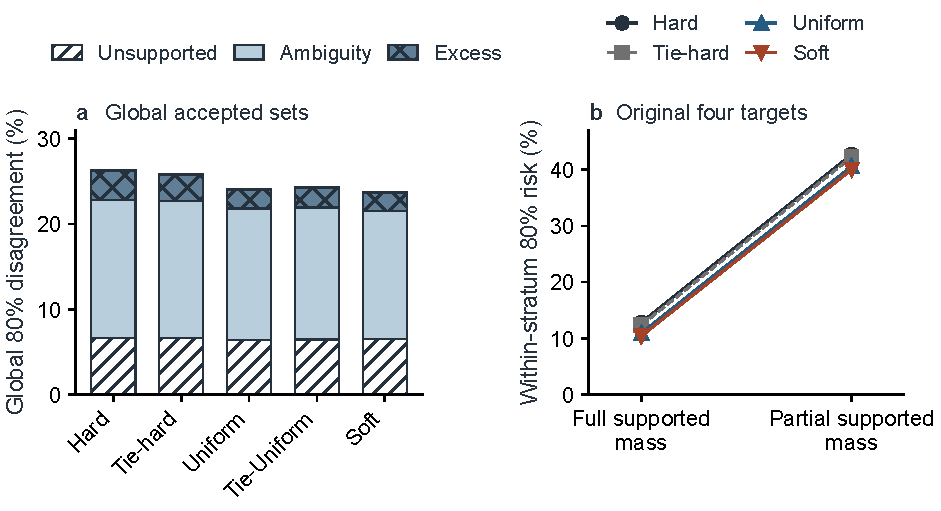
\includegraphics[width=\linewidth]{submission_reader_2026_10_13/source/figures/Fig3.pdf}
\caption{Risk components at 80\% coverage. (a) All five Swin-T targets on each model's global accepted set. (b) The original four targets with selection performed separately within the full- and partial-supported-mass strata. Panels use different populations and vertical scales. Zero-supported-mass images have complete-vote disagreement one; their acceptance counts appear in Table~\ref{tab:retention}. Unsupported votes remain in every score}\label{fig:mass}
\end{figure}

Overall risk also conceals differences in which unsupported images are accepted. Soft accepts a mean 11.00 of the 16 zero-supported-mass images, compared with 7.00 for Uniform and 6.67 for Tie-Uniform (Table~\ref{tab:retention}). Its lower overall disagreement therefore does not imply more effective rejection of these images. The counts are small and descriptive, rather than estimates of a deployment failure rate. The supplement reports contempt, unknown and not-a-face vote mass separately because these categories have different meanings, including all-image and accepted-set summaries for calibration and testing.
\begin{table}[t]
\caption{Accepted image counts at global 80\% coverage, seeds 17, 42, 89 in that order. Population sizes: full 1,732; partial 1,527; zero 16}\label{tab:retention}
\centering\begin{tabular}{lrrr}\toprule
Targets & Full mass & Partial mass & Zero mass\\\midrule
Hard & 1499, 1501, 1492 & 1115, 1112, 1122 & 6, 7, 6\\
Tie-hard & 1519, 1494, 1508 & 1092, 1119, 1106 & 9, 7, 6\\
Uniform & 1515, 1527, 1527 & 1098, 1087, 1085 & 7, 6, 8\\
Tie-Uniform & 1529, 1522, 1520 & 1084, 1090, 1095 & 7, 8, 5\\
Soft & 1527, 1527, 1533 & 1081, 1083, 1076 & 12, 10, 11\\
\bottomrule\end{tabular}\par
Each seed retains 2,620 images in total. Zero-mass images have disagreement one under every supported prediction.
\end{table}


\subsection{Sensitivity to confidence scores}
\begin{table}[t]
\caption{Exploratory score sensitivity at 80\% coverage: paired-seed mean Soft-minus-control disagreement (pp). Negative values favor Soft; accepted image sets can differ}\label{tab:scores}
\centering\begin{tabular}{lllrr}\toprule
Backbone & State & Score & Uniform & Tie-Uniform\\\midrule
Swin-T & Selected & MSP & -0.378 & -0.588\\
Swin-T & Selected & Margin & -0.153 & -0.299\\
Swin-T & Selected & Neg. entropy & -0.093 & -0.323\\
Swin-T & Epoch 12 & MSP & -0.317 & -0.307\\
Swin-T & Epoch 12 & Margin & -0.122 & -0.057\\
Swin-T & Epoch 12 & Neg. entropy & -0.296 & -0.242\\
ResNet-18 & Selected & MSP & +0.173 & +0.042\\
ResNet-18 & Selected & Margin & +0.417 & +0.206\\
ResNet-18 & Selected & Neg. entropy & +0.509 & +0.485\\
ResNet-18 & Epoch 12 & MSP & +0.170 & +0.190\\
ResNet-18 & Epoch 12 & Margin & +0.511 & +0.555\\
ResNet-18 & Epoch 12 & Neg. entropy & +0.307 & +0.435\\
\bottomrule\end{tabular}\par
\smallskip
MSP reproduces the original ledger exactly. Margin and negative entropy are post hoc sensitivity analyses, not proposed rejection methods. Per-seed results are in Table~S14 and Fig.~S7.\par
\end{table}
The exploratory score analysis retains the mean direction of the backbone-specific comparison at 80\% coverage, but not its magnitude (Table~\ref{tab:scores}). Validation-selected Swin-T favors Soft under MSP, margin and negative entropy, while the corresponding ResNet-18 means favor Uniform. Some individual Swin-T seed contrasts under margin or entropy nevertheless favor Uniform; the supplementary per-seed table shows these reversals. Thus, the average direction at this endpoint is not solely a consequence of using MSP, but neither the score nor the supervision target has a uniform advantage across configurations. At full coverage the three scores give identical risk, since they no longer change the accepted set. These probability-only checks do not compare learned rejection methods.


\subsection{Calibration-to-test transfer}
Empirical thresholds do not preserve their nominal risk targets when transferred unchanged from calibration to testing. Across the original four conditions, all 36 nonempty empirical test settings exceed their targets (Table~\ref{tab:policies}). These settings overlap and are not independent Bernoulli trials. At the 10\% target, Soft attains greater mean coverage than Hard (49.54\% versus 38.35\%), but also greater achieved risk (13.01\% versus 11.45\%). The coverage difference is therefore not a comparison at equal risk.
\begin{table}[t]
\caption{Calibration-fitted policies applied unchanged to primary testing. Entries are mean coverage / risk (\%); coverage includes empty seeds, risk averages nonempty seeds}\label{tab:policies}
\centering\begin{tabular}{llcc}\toprule
Risk target & Supervision & Empirical & Fixed-grid bound\\\midrule
10\% & Hard & 38.35 / 11.45 (3/3) & 0.00 / -- (0/3)\\
10\% & Tie-hard & 39.17 / 11.93 (3/3) & 0.00 / -- (0/3)\\
10\% & Uniform & 45.99 / 12.22 (3/3) & 0.00 / -- (0/3)\\
10\% & Soft & 49.54 / 13.01 (3/3) & 0.00 / -- (0/3)\\
\addlinespace
20\% & Hard & 68.58 / 22.28 (3/3) & 47.03 / 14.55 (3/3)\\
20\% & Tie-hard & 71.04 / 22.80 (3/3) & 48.05 / 14.61 (3/3)\\
20\% & Uniform & 76.20 / 22.80 (3/3) & 57.49 / 16.11 (3/3)\\
20\% & Soft & 76.88 / 22.56 (3/3) & 60.39 / 16.60 (3/3)\\
\addlinespace
30\% & Hard & 98.06 / 32.39 (3/3) & 82.01 / 26.92 (3/3)\\
30\% & Tie-hard & 99.47 / 32.37 (3/3) & 85.41 / 27.54 (3/3)\\
30\% & Uniform & 99.94 / 31.46 (3/3) & 88.41 / 27.11 (3/3)\\
30\% & Soft & 99.91 / 31.07 (3/3) & 89.57 / 27.01 (3/3)\\
\bottomrule\end{tabular}\par
\smallskip\par\footnotesize Parentheses give nonempty test seeds. An empty policy has undefined risk. Neither a nominal target nor the bound's unverified independence/unchanged-population assumptions establish a deployment guarantee. Different achieved risks are not an equal-risk coverage comparison.
\end{table}


The calibration and test populations differ even before confidence selection. Their annotation floors are 23.70\% and 26.67\%, respectively, a +2.97 pp difference; unsupported mass rises from 5.72\% to 7.88\%, with the remainder due to supported-category ambiguity. Figure~\ref{fig:transfer} applies the same accounting to the accepted sets. For Soft at the nominal 20\% target, the +2.57 pp test-minus-calibration risk gap comprises +1.98 pp unsupported mass, +0.78 pp supported ambiguity and -0.19 pp excess. These components describe the gap rather than independent causes.
\begin{figure}[tp]
\centering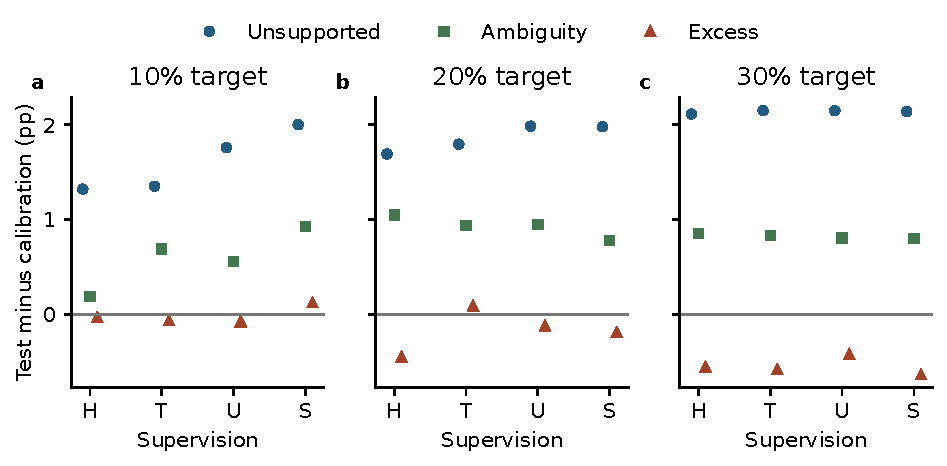
\includegraphics[width=\linewidth]{submission_reader_2026_10_13/source/figures/Fig6.pdf}
\caption{Mean test-minus-calibration differences in unsupported mass, supported ambiguity and excess disagreement for empirical thresholds. Components sum to the risk gap. H: Hard; T: Tie-hard; U: Uniform; S: Soft. The three risk-target panels share a vertical scale. Means use paired nonempty calibration/test accepted sets}\label{fig:transfer}
\end{figure}

The additional diagnostics distinguish variability within calibration from the coverage cost of a more conservative rule. At the 20\% target, calibration-half-split holdout-minus-fit gaps average +0.05 to +0.19 pp across conditions, with broad descriptive 5th--95th-percentile ranges of roughly -2.3 to +2.8 pp. The supplement retains complete per-condition resamples. These summaries do not uniquely separate distribution shift, finite-sample fluctuation and threshold-search effects. The fixed-grid comparator yields 24 nonempty test settings, with 0 exceeding their nominal targets, but rejects every image at the 10\% target for every condition and seed. Its observed conservatism has a concrete coverage cost and does not verify its population assumptions.

\subsection{External clip evaluation and diagnostic analyses}

All 1,440 external clips and 11,520 sampled frames meet the frozen eligibility rules, giving 100\% maximum achievable coverage without model-outcome filtering. Table~\ref{tab:external} summarizes disagreement for both backbones, checkpoint states and annotation references. Changing the reference from raw responses to calm/neutral-merged responses scores the same predictions and accepted clips; it does not change inference or selection.

\begin{table}[t]
\caption{External disagreement at 80\% MSP coverage (\%): means of three seed-specific risks, not an ensemble. Every model accepts its own 1,152 of 1,440 clips}\label{tab:external}
\centering\small\begin{tabular}{lllrrr}\toprule
Backbone & State & Reference & Soft & Uniform & Tie-Uniform\\\midrule
Swin-T & Selected & Raw & 68.37 & 67.75 & 67.42\\
Swin-T & Selected & Merged & 60.72 & 60.62 & 60.03\\
Swin-T & Epoch 12 & Raw & 68.25 & 68.03 & 67.45\\
Swin-T & Epoch 12 & Merged & 60.47 & 61.37 & 60.16\\
ResNet-18 & Selected & Raw & 71.49 & 69.66 & 70.73\\
ResNet-18 & Selected & Merged & 63.20 & 61.88 & 62.46\\
ResNet-18 & Epoch 12 & Raw & 71.32 & 69.62 & 70.47\\
ResNet-18 & Epoch 12 & Merged & 63.24 & 61.96 & 62.35\\
\bottomrule\end{tabular}\par\smallskip
Raw retains nine human responses; Merged adds calm to neutral and retains none. Neither is intended-expression accuracy. The model predictions and accepted IDs are unchanged between references.\par
\end{table}

\begin{table}[t]
\caption{Principal external comparison: validation-selected Swin-T Soft minus Uniform at 80\% MSP coverage (percentage points). Negative favors Soft}\label{tab:externalseeds}
\centering\small\begin{tabular}{lrrrrl}\toprule
Reference & Seed 17 & Seed 42 & Seed 89 & Mean & Actor interval\\\midrule
Raw & -0.052 & +2.639 & -0.755 & +0.611 & [+0.23, +1.09]\\
Merged & -1.276 & +2.483 & -0.903 & +0.101 & [-0.26, +0.59]\\
\bottomrule\end{tabular}\par\smallskip
Percentile 95\% actor-cluster intervals use shared actor multiplicities and reranking within 5,000 replicates, conditional on these three fitted pairs and observed votes. They do not quantify seed-population, new-rater or unrestricted demographic uncertainty.\par
\end{table}

The principal external contrast does not reproduce the source-dataset advantage consistently across seeds (Table~\ref{tab:externalseeds}). Under the raw reference, the +0.611 pp mean is driven by the larger positive contrast for seed 42, which outweighs the negative contrasts for seeds 17 and 89. Its actor-cluster interval lies above zero, but describes actor-sampling sensitivity conditional on these fitted pairs and observed votes. Under the merged reference, the interval crosses zero. Neither result establishes equivalence or a stable external ordering across retraining.

Checkpoint state and annotation reference further qualify the comparison. Under the merged reference, all three epoch-12 Swin-T contrasts favor Soft, whereas the validation-selected contrasts have mixed directions. The complete per-seed results remain in the supplement. The external evaluation therefore tests the transfer of the frozen pipelines as a whole; it does not isolate supervision from differences in capture conditions, population or frame aggregation.

\begin{figure}[tp]\centering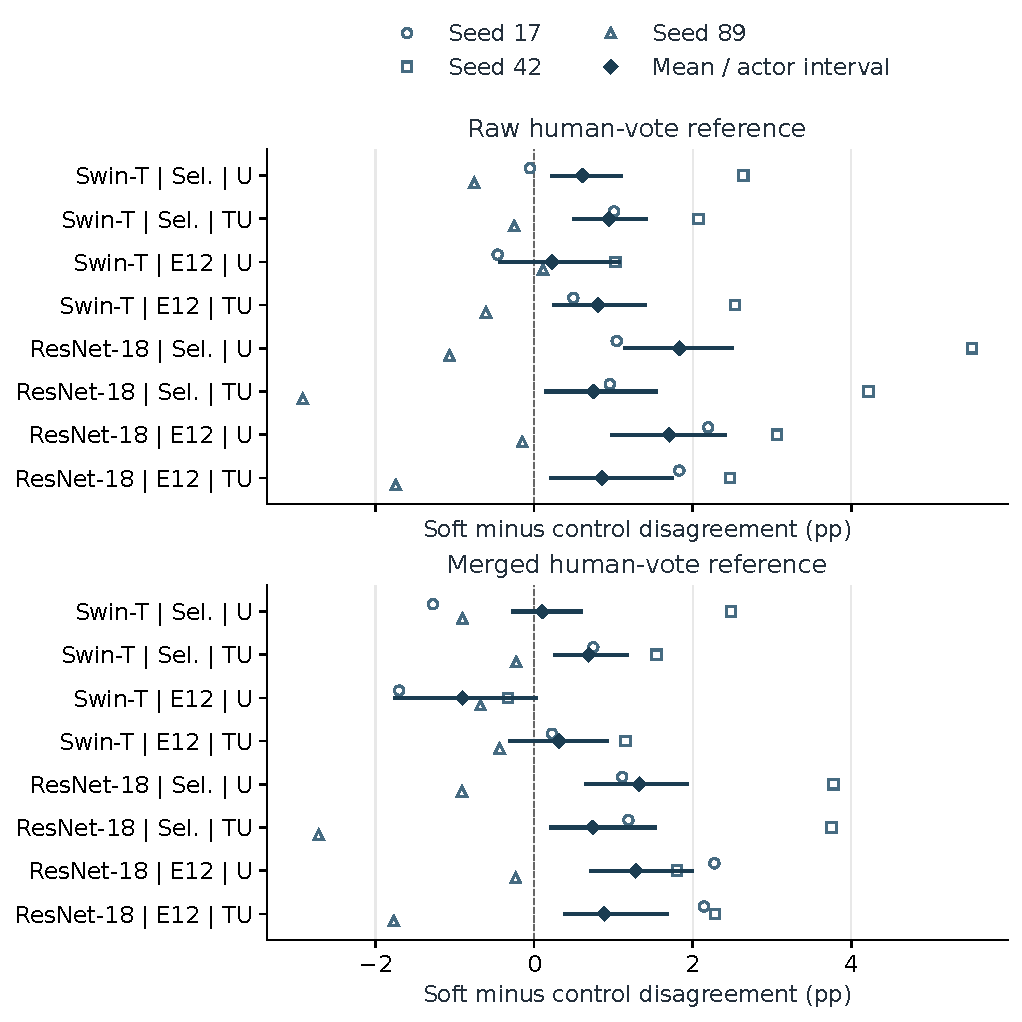
\includegraphics[width=\linewidth]{submission_reader_2026_10_13/source/figures/ExternalContrasts.pdf}

\caption{External disagreement differences at 80\% MSP coverage, using separate model rankings. Hollow symbols show all three paired seed contrasts; the diamond and bar show their mean and conditional 95\% actor-cluster interval. Vertical offsets separate the seeds. Sel.: selected checkpoint; E12: fixed-epoch checkpoint; U: Uniform; TU: Tie-Uniform. Both panels share the horizontal scale; negative favors Soft. Intervals describe actor-sampling sensitivity for these fitted pairs and votes, not uncertainty over new seeds, raters or populations. Zero denotes equal mean disagreement, not equivalent predictions or accepted sets}\label{fig:external}\end{figure}

\begin{table}[htbp]
\caption{Principal external risk accounting: validation-selected Swin-T, means across three seeds (\%). Components use the same population as total risk}\label{tab:externalaccounting}
\centering\small\begin{tabular}{lllrrrr}\toprule
Population & Supervision & Ref. & Risk & Unsup. & Ambig. & Excess\\\midrule
All eligible & Soft & Raw & 71.06 & 11.90 & 16.81 & 42.36\\
All eligible & Uniform & Raw & 70.81 & 11.90 & 16.81 & 42.11\\
All eligible & Soft & Merged & 64.84 & 3.14 & 20.23 & 41.47\\
All eligible & Uniform & Merged & 64.81 & 3.14 & 20.23 & 41.44\\
80\% MSP & Soft & Raw & 68.37 & 14.00 & 16.61 & 37.76\\
80\% MSP & Uniform & Raw & 67.75 & 13.58 & 16.59 & 37.58\\
80\% MSP & Soft & Merged & 60.72 & 3.31 & 20.78 & 36.64\\
80\% MSP & Uniform & Merged & 60.62 & 3.30 & 20.57 & 36.75\\
\bottomrule\end{tabular}\par\smallskip
All eligible: 1,440 clips per state. 80\% MSP: 1,152 independently ranked clips per state. Unsup. is unsupported vote mass; Ambig. is supported ambiguity. All-eligible components are not substituted for accepted-set components. Rounding can prevent displayed components from summing exactly.\par
\end{table}

The risk accounting identifies excess disagreement as the largest component both across all eligible clips and at 80\% MSP coverage (Table~\ref{tab:externalaccounting}). For validation-selected Swin-T Soft under the raw reference, the all-eligible excess is 42.36 percentage points, compared with 11.90 points of unsupported vote mass. Missing output categories alone therefore do not explain the poor transfer. The decomposition describes disagreement rather than its cause, and accepted-set components must be read on their own population rather than substituted from all-eligible averages.

The post hoc diagnostics show that neutral dominates accepted predictions in all three validation-selected Swin-T seeds: 67.0--70.0\% for Soft and 62.7--68.3\% for Uniform. The supplementary vote-weighted matrices and temporal summaries retain all six principal matrices and all eight temporal bins. Neutral probability is highest in the first bin and falls toward the middle, while frame-to-clip argmax agreement also varies across bins. These patterns describe the frozen outputs; they do not establish a cause of transfer failure or measure frame accuracy, since the human judgments apply to whole clips.

Online Resource 8 retains all 36 external states, category frequencies, raw-reference vote mass, raw/merged matrices and temporal summaries. The supplementary score/coverage and fixed-image comparisons provide the complete sensitivity results without changing the primary external comparison.

